% A Bernoulli Evolutionary Strategy for Binary Weight Neural Network Optimization
% EvoStar 2027 (EvoApplications track) submission.
%
% Build: pdflatex total && bibtex total && pdflatex total && pdflatex total
%
% TODO before submission:
%   - author names, affiliations, ORCIDs (search "TODO")
%   - acknowledgments / funding
%   - code/data URL for the reproducibility statement
%   - refs.bib must contain liu2021adam (cited in the Introduction)
\documentclass[runningheads]{llncs}

\usepackage[T1]{fontenc}
\usepackage{graphicx}
\usepackage{amsmath}
\usepackage{amssymb}
\usepackage{booktabs}
%
% If you use the hyperref package, please uncomment the following two lines
% to display URLs in blue roman font according to Springer's eBook style:
%\usepackage{color}
%\renewcommand\UrlFont{\color{blue}\rmfamily}
%\urlstyle{rm}
%
\graphicspath{{figures/}}

\begin{document}

\title{A Bernoulli Evolutionary Strategy for Binary Weight Neural Network Optimization}

%\titlerunning{Evolutionary Strategies for Binary Neural Network Optimization}

% TODO: real author names, ORCIDs and institutes
\author{}
\authorrunning{}
\institute{}

\maketitle

\begin{abstract}
Training binary weight neural networks is complicated by the fact that the
parameters are not continuous, and so standard gradient descent does not
directly apply. Typically this problem is solved by storing continuous
surrogate parameters that are quantized during the forward and backward
passes. The surrogate parameters are then updated with the gradient instead
of the quantized parameters, which works well in practice when done in
conjunction with an optimizer like Adam, and with gradient and weight
clipping. A number of interpretations for what these surrogate parameters
represent have been suggested, including inertia and Bernoulli
expectations. Considering this, an alternative approach to training such
models could be a gradient-approximation algorithm such as an evolutionary
strategy that optimizes a distribution over quantized parameterizations.
In this work we derive a Bernoulli evolutionary strategy for optimizing
binary weight neural networks, which avoids backpropagation entirely, and
use MNIST digit classification as a means of exploring the behavior of the
algorithm. We perform a sweep over population sizes and measure performance
and distribution entropy at each model layer, finding that test accuracy
grows with population size, while larger populations retain higher
distribution entropy throughout training. We also find that the
output layer distributions saturate faster than other layers. We train the
same network architecture with the straight-through estimator approach
using the Adam optimizer, and find that our algorithm reaches similar
performance. Our results suggest that evolutionary strategies can train
quantized neural networks, and we discuss extensions to non-differentiable
architectures more broadly and distributed training.
% TODO before submission: add code URL to the reproducibility statement.
\keywords{Binary Weight Neural Networks \and Evolutionary Strategies \and Quantization}
\end{abstract}

\section{Introduction}
\label{sec:intro}

The application of a model in a given domain depends on the available compute relative to the cost of model inference. But the training of said model with deep learning has to account for the cost of calculating gradients and maintaining optimizer states. Attempts to mitigate the cost of model inference by reducing the bits required per parameter have been made frequently in the literature, and generally are characterized as quantization techniques. But the binary weight neural network, where each parameter is stored in a single bit, reduces the per-parameter memory overhead as much as possible, reducing memory and bandwidth bottlenecks
\cite{courbariaux2016binarized,rastegari2016xnor,yuan2023survey}. Although desirable for inference properties, such models are inherently problematic when it comes to training, since backpropagation tends to rely on continuous gradients. The typical solution to training comes from the use of the straight-through-estimator, where surrogate continuous parameters are stored for each binary one, and gradients are followed in this continuous space instead of the binary space \cite{bengio2013estimating}. Practically this approach works very well when combined with techniques to minimize the problem of exploding gradients, normally batch normalization or some pre-activation scaling factor
\cite{sari2019batchnorm}, and an optimizer like Adam \cite{liu2021adam,kingma2015adam}.

When it was found that binary weight neural networks could be trained in this way works were largely unprincipled and empirically validated. Helwegen et al. came to suggest that surrogate parameters could be viewed as inertia acting on the binary parameters, and suggested an optimizer based on this concept that functions well \cite{helwegen2019latent}. Meng et
al.~\cite{meng2020bayesian} suggest using the Bayesian learning rule, and that the surrogate parameters encode the Bernoulli expectation for each binary parameter and derive an algorithm that
justifies several empirically justified choices from the literature. Notably, in their work they suggest that a REINFORCE gradient estimate could be used to learn these expectations, but do not explore this idea any further. In their work on evolutionary strategies Salimans et al. also suggest that the evolutionary strategy approach lends itself to optimization of binary weight neural networks, and networks with non-differentiable architectures \cite{salimans2017evolution}.

In this work we look to take a first step toward understanding the applicability of evolutionary strategies for this purpose by deriving an algorithm for optimizing binary weight neural networks. We use a scaling factor for ReLU based networks that replaces batch normalization layers, particularly useful for evolutionary strategies that otherwise require techniques like virtual batch normalization. Next we look at how population size impacts performance and convergence, finding that test accuracy improves with increasing population size but at a decreasing rate. Finally, we compare the performance of our algorithm to a straight-through-estimator approach using the Adam optimizer, finding that our approach reaches similar performance.

\section{Binary Weight Neural Networks}
\label{sec:BWNN}

\subsection{Efficient Forward Pass}
\label{sec:bwnn:forward}

A binary weight neural network stores every weight in a single bit. We
write the stored parameters as a binary vector $x \in \{0,1\}^{D}$ and
obtain the usable weights through the sign map $w = 2x - 1 \in
\{-1,+1\}^{D}$; a layer with fan-in $n$ computes pre-activations
\begin{equation}
y = \gamma\, W a,
\qquad W \in \{-1,+1\}^{m \times n},
\label{eq:bwnn-layer}
\end{equation}
where $a$ is the input to the layer and $\gamma$ a fixed per-layer scale
justified below. Storing $W$ bit-wise compresses the
parameters by up to $32\times$ relative to float32, which is what makes
these models attractive for memory-constrained deployment
\cite{courbariaux2016binarized,rastegari2016xnor,yuan2023survey}.

We have found that deep networks of binary parameters with ReLU
activations do not train well, which corroborates with findings in the
literature. The standard approach is to apply batch normalization, but
this introduces a problem for evolutionary strategies since each member
of the population needs independent batch normalization statistics.
Salimans et al.\ addressed this issue with virtual batch normalization
\cite{salimans2017evolution}, where a hold-out batch is maintained
exclusively to update the batch normalization layers, and fitness is
calculated only after updating these layers first on the hold-out set.
Work on binary weight neural networks with sign activation functions has
shown that the batch normalization layer can be replaced by a constant
scaling factor without much cost in model performance
\cite{sari2019batchnorm}. Our networks use the ReLU activation function,
and so we replace batch normalization with a scaling factor of
$\sqrt{2}/\sqrt{n_{in}}$ (the scale $\gamma$ of
Eq.~\ref{eq:bwnn-layer}), which we apply after each hidden layer. Without scaling neurons are able to reach very large values that disrupt training in both gradient and gradient approximation settings.

\section{Bernoulli Evolutionary Strategy}
\label{sec:BES}

Consider the binary parameter vector $x \in \{0,1\}^{D}$. Where gradient-based methods maintain a point
estimate in a continuous parameter space, we instead maintain a
distribution over binary vectors and optimise the parameters of that
distribution.

We use independent Bernoulli distributions to sample each parameter. Each bit carries a real-valued logit $\theta_j$ with
\begin{equation}
p(x_j = 1 \mid \theta_j) = s_j, \qquad
s_j = \sigma(\theta_j) = \frac{1}{1 + e^{-\theta_j}},
\label{eq:bes-bern}
\end{equation}
so the probability of a full parameter vector factorises as
\begin{equation}
p(x \mid \theta) = \prod_{j=1}^{D} s_j^{\,x_j}\,(1-s_j)^{\,1-x_j}.
\label{eq:bes-factor}
\end{equation}
When $\theta_j = 0$ the belief is that parameter $j$ takes a value of 1 with probability $0.5$. We assume no prior belief about the appropriate state of each parameter, so initialize the search parameters to 0.

Let $f : \{0,1\}^D \to \mathbb{R}$ denote a scalar fitness, with higher
values being better. The quantity we optimise is the expected fitness under
the search distribution,
\begin{equation}
J(\theta) = \mathbb{E}_{x \sim p(x \mid \theta)}\bigl[f(x)\bigr]
          = \sum_{x} f(x)\, p(x \mid \theta).
\label{eq:bes-objective}
\end{equation}
$J$ is a smooth function of $\theta$ even though $f$ is defined only on
a discrete set: the randomness of the sampling does the smoothing. Its
gradient is
\begin{align}
\nabla_\theta J(\theta)
  &= \sum_{x} f(x)\, \nabla_\theta p(x \mid \theta)
   = \sum_{x} f(x)\, p(x \mid \theta)\,
     \nabla_\theta \log p(x \mid \theta)
     \nonumber\\
  &= \mathbb{E}_{x \sim p(x \mid \theta)}
     \bigl[f(x)\, \nabla_\theta \log p(x \mid \theta)\bigr],
\label{eq:bes-score}
\end{align}
where the second step uses the identity
$\nabla_\theta p = p\,\nabla_\theta \log p$. This is the
likelihood-ratio, or REINFORCE, estimator
\cite{williams1992simple,bengio2013estimating}: the fitness, which is
not necessarily differentiable, appears only as a multiplicative weight, while the
score function $\nabla_\theta \log p(x \mid \theta)$ is known exactly.

Taking the
logarithm of \eqref{eq:bes-factor},
\begin{equation}
\log p(x \mid \theta) = \sum_{j=1}^{D}
  \bigl[x_j \log s_j + (1 - x_j) \log (1 - s_j)\bigr],
\label{eq:bes-loglik}
\end{equation}
the $j$-th coordinate of the score depends only on $x_j$ and $\theta_j$.
Differentiating \eqref{eq:bes-loglik} with respect to the logit, using
the logistic derivative $\sigma'(\theta_j) = s_j(1-s_j)$,
\begin{equation}
\frac{\partial \log p(x \mid \theta)}{\partial \theta_j}
  = \frac{x_j - s_j}{s_j(1-s_j)} \cdot s_j(1-s_j)
  = x_j - s_j,
\label{eq:bes-score-bit}
\end{equation}
the Fisher denominator of the Bernoulli parameterisation cancels exactly
under the logit reparameterisation, and the score reduces to
\begin{equation}
\nabla_\theta \log p(x \mid \theta) = x - s,
\qquad s = \sigma(\theta).
\label{eq:bes-score-vec}
\end{equation}

In our derivation we omit consideration of fitness shaping for convenience, but the standard approach is that the raw fitness score is replaced by another function dependent on $f$ that changes convergence dynamics. The classic approach is to subtract a baseline from the fitness scores, such as an exponential moving average of population fitness, but other approaches like rank based fitness shaping are also used to mitigate early convergence. In our work we compare rank shaping and standard shaping.

The expectation \eqref{eq:bes-score} is estimated with a population of
$P$ i.i.d.\ individuals $x_1, \dots, x_P \sim p(x \mid \theta)$, each
evaluated once by the fitness function. Writing $u_i$ for the shaped fitness of individual $i$,
the population-summed update applied to each coordinate is
\begin{equation}
\theta_j \leftarrow \theta_j + \frac{\eta}{P} \sum_{i=1}^{P} u_i\,(x_{ij} - s_j),
\label{eq:bes-update}
\end{equation}
with learning rate $\eta$.

\section{Methods}
\label{sec:methods}

Our experiments are conducted on the MNIST digit classification dataset \cite{lecun1998gradient}, where we take 6000 of the 60000 training images and keep them for validation. The 10000 image test set is kept separate. We subtract the training set mean and std from all input data. In all our experiments we use a fully connected multilayer perceptron with 2 hidden layers of 256 neurons each. We use a ReLU activation function with pre-activation scaling in each layer as previously described, and no biases. Our fitness function is negative categorical cross-entropy on random mini-batches of size 4096. At checkpoints during training we record the performance of the mode network, that is we take the most likely binary parameters given the search distribution and evaluate them. Every 10 iterations we measure validation accuracy, and measure test accuracy at the end of training. We found that keeping a constant learning rate of $\eta = 100$ performed well for all studied configurations, likely being so large thanks to the division by the population size in the gradient approximation. Our fitness shaping function is centered average ranks in the range [-0.5, 0.5]. The search distribution is initialized to 0, so that each parameter has equal probability of being sampled as -1 or 1 in the first iteration. We track the average entropy across the search distribution. In our STE experiments we employ the Larq Tensorflow package, using quantized \texttt{ste\_sgn} weights and the same architecture as previously described otherwise. For all our experiments we train over 5 seeds. Our population size experiments were performed for 2000 iterations, while the trace, histogram, and comparison with STE were performed for 5000 iterations. Our Adam baseline is from 100 epochs of training with batch size 512 and learning rate $10^{-3}$.

\section{Results}
\label{sec:results}

\begin{figure}
    \centering
    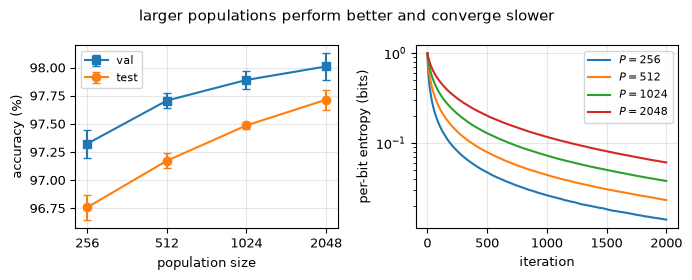
\includegraphics[width=1\linewidth]{fig_pop_scaling.png}
    \caption{Increasing the population size leads to improved validation and test accuracy in our experiments. Larger population sizes also lead to search distributions that converge slower despite their improved performance.}
    \label{fig:popsize}
\end{figure}

Fig.~\ref{fig:popsize} shows accuracy and average search distribution entropy varying population size. We see two clear trends from this figure: accuracy increases as the population size increases, and the population converges slower as the population size increases. It appears that the population size improves performance less as it increases, which is consistent with literature in continuous optimization with evolutionary strategies. The entropy curves show that large populations lead to less convergence in the same number of iterations, and consequently can produce more diverse populations.

\begin{figure}
    \centering
    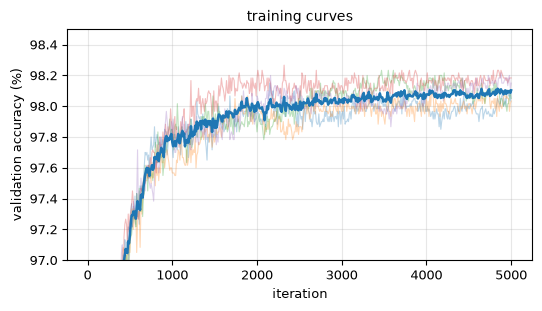
\includegraphics[width=1\linewidth]{fig_val_traces.png}
    \caption{Training curves over 5 seeds, along with the average curve in blue. Since these curves correspond to the validation accuracy of the search distribution mode network, their positive trend and volatility suggest that optimizations could be made to the algorithm in this later stage of training. Similar findings were reported in early literature on binary neural network training.}
    \label{fig:traces}
\end{figure}

Fig.~\ref{fig:traces} shows training curves across 5 seeds along with the average curve. The search distribution consistently reaches high validation accuracy before performance gains slow considerably. It is also clear that although the curves trend upward they are highly volatile. The validation accuracy is calculated using the mode network, i.e. the most likely binary parameters, which implies that there is substantial variance in the fitness across sampled populations even when most of the search distribution has converged.

\begin{figure}
    \centering
    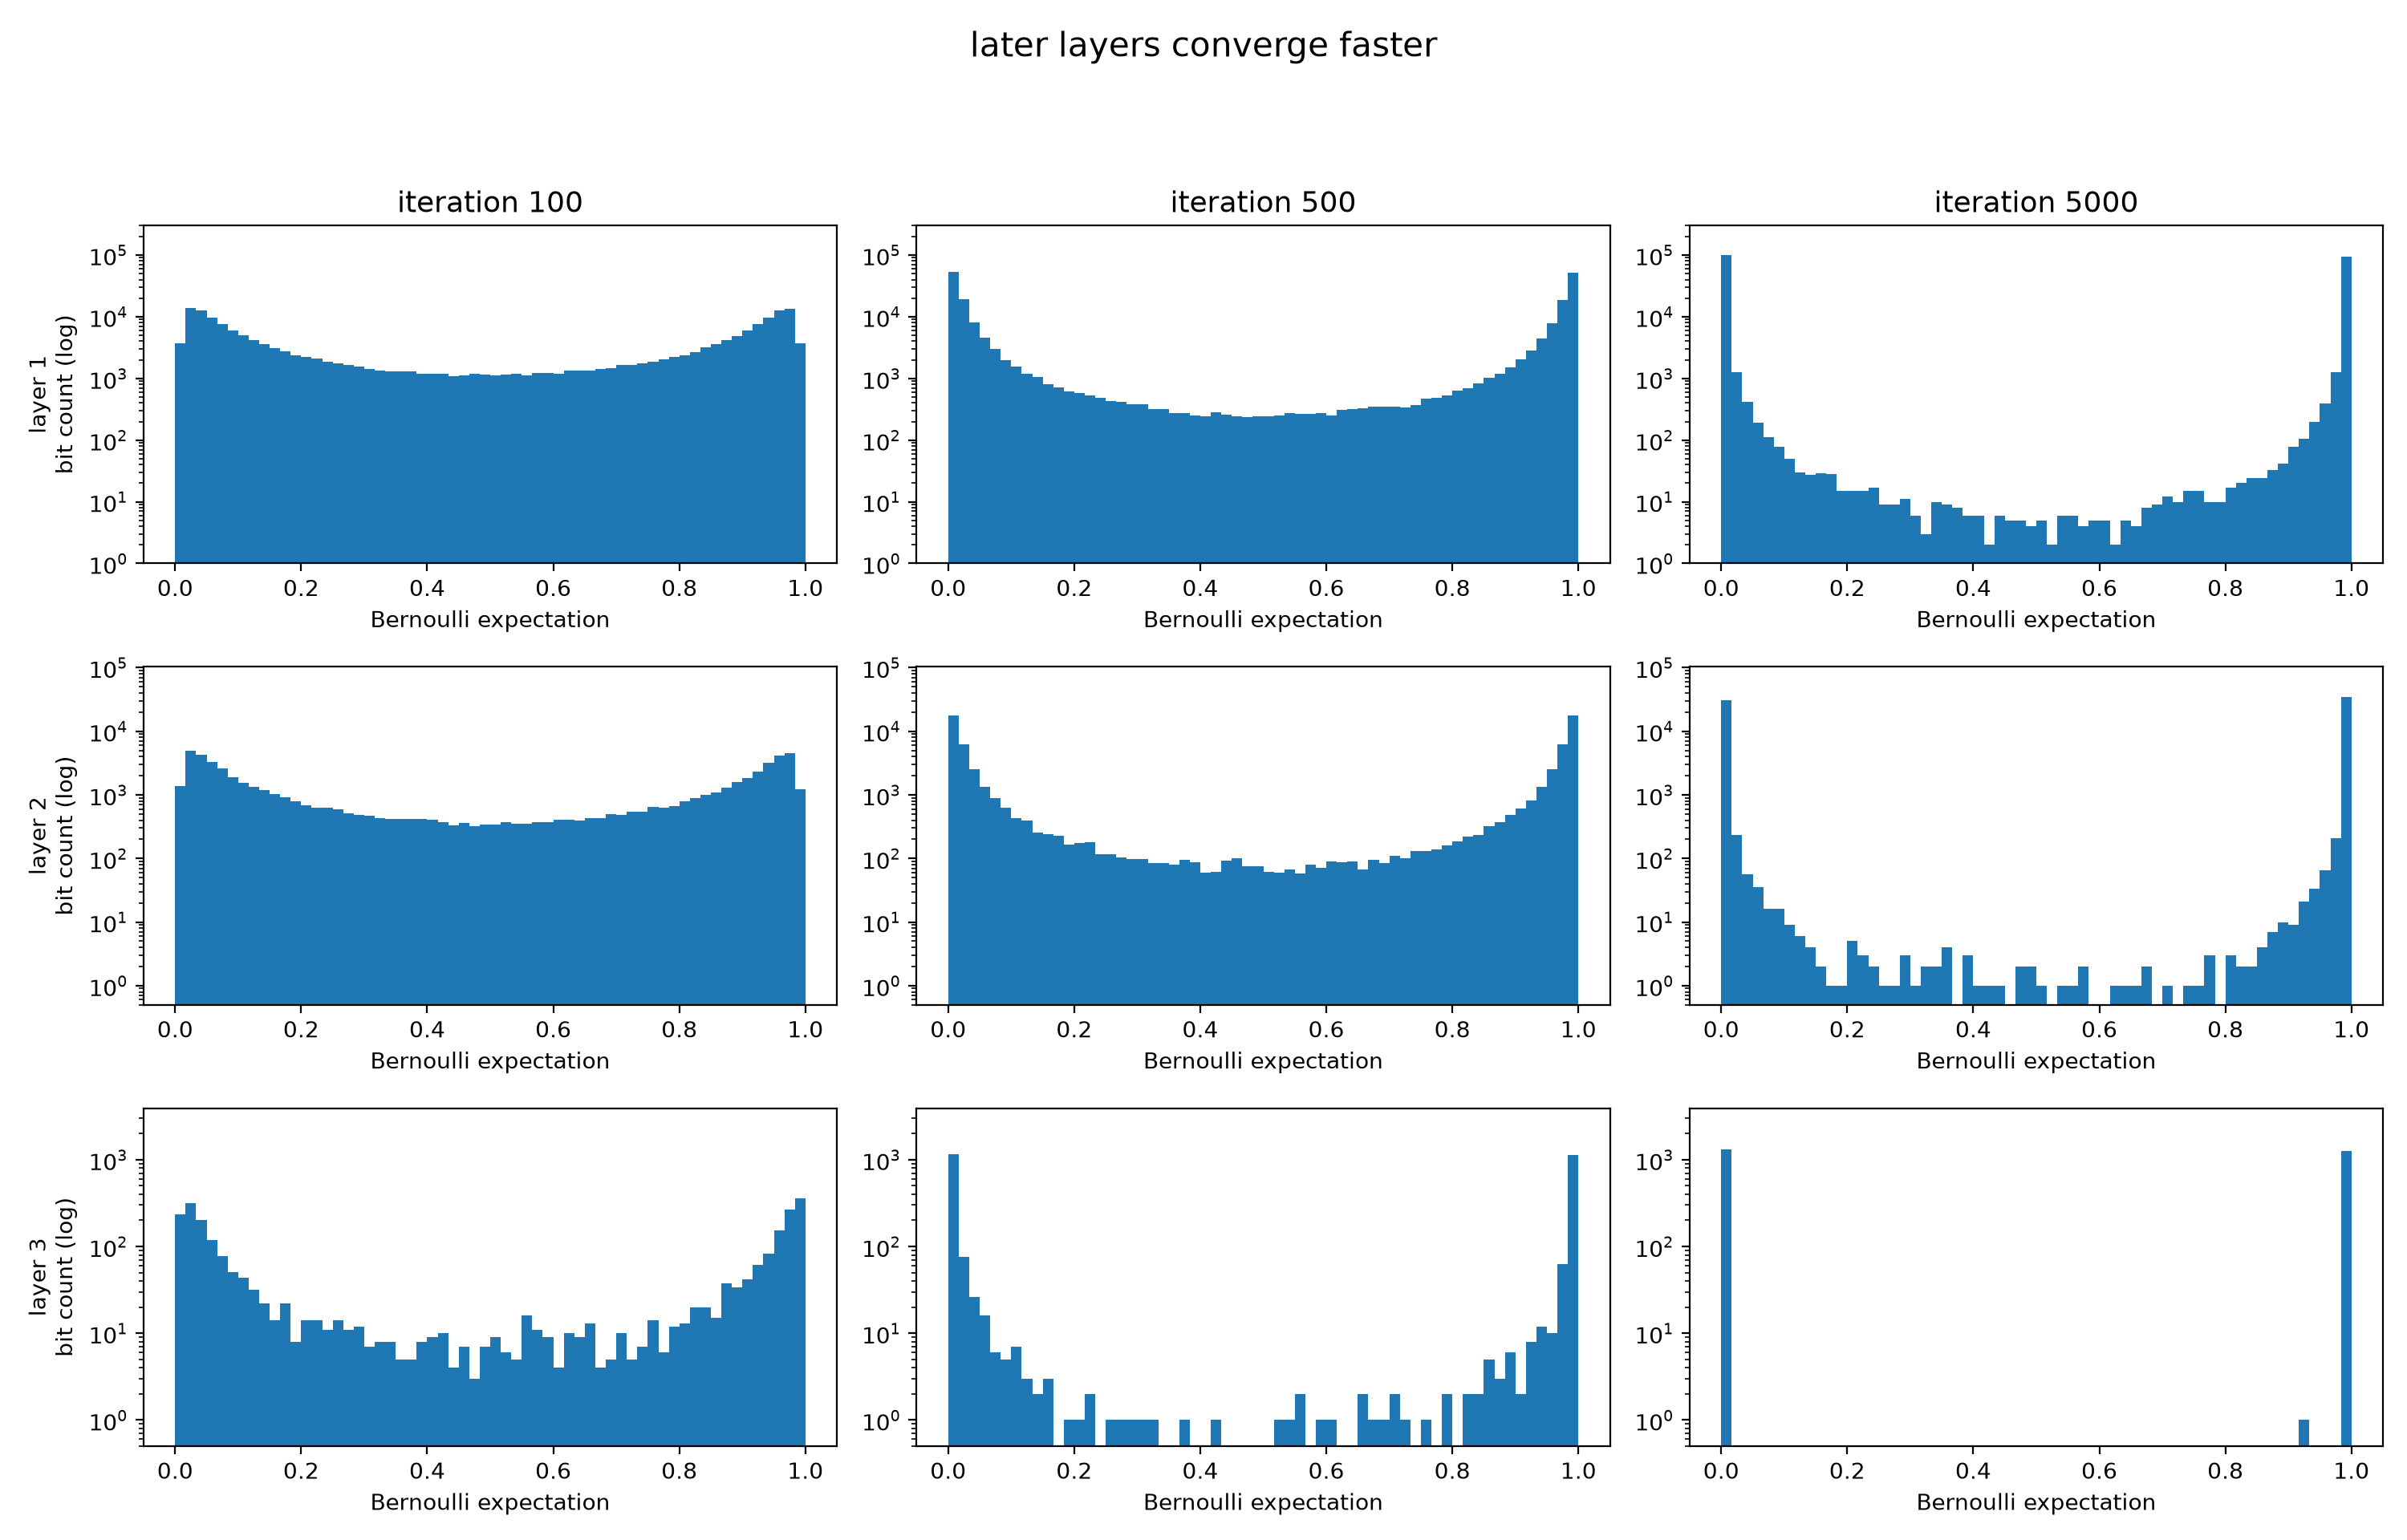
\includegraphics[width=1\linewidth]{theta_expectations_layers_h256x2_p2048_seed42.png}
    \caption{Histograms of Bernoulli expectations from each layer of the network search distribution at different points in training. It is clear that the output layer has converged far faster than the other layers.}
    \label{fig:hists}
\end{figure}

Fig.~\ref{fig:hists} shows the distribution of Bernoulli expectations across the layers of a network at different points during training. Each layer demonstrates a similar pattern where most of the distributions saturate, but the depth of the layer changes how quickly. Notably, the output layer has essentially converged by iteration 5000, but we know that there is still volatility in the validation accuracy at this iteration. There are two potential explanations for this behaviour. The first is that the layer order also corresponds to the number of parameters in the network, so that the first layer has the most, and the output the least. Considering layers as independent optimization problems it seems plausible that convergence would be quicker in the smaller search space. Alternatively, it could have to do with the proximity to the fitness signal, in the sense that output layer parameters directly manipulate logits, and thus the classification distribution.

\begin{table}[t]
\centering
\caption{Bernoulli ES vs.\ Adam-STE (5 Seeds)}
\label{tab:es-ste}
\begin{tabular}{lcc}
\toprule
Method & val acc (\%) & test acc (\%) \\
\midrule
Bernoulli ES & $98.10 \pm 0.06$ & $97.87 \pm 0.07$ \\
STE + Adam & $98.16 \pm 0.27$ & $98.02 \pm 0.30$ \\
\bottomrule
\end{tabular}
\end{table}

Table~\ref{tab:es-ste} shows a comparison over 5 seeds of our algorithm and a standard gradient approach. Our algorithm reaches performance within the margin of error of the gradient approach, albeit slightly lower than the average. We suspect that with additional techniques standard in evolutionary strategy literature, such as antithetic sampling, the performance of our algorithm could match that of the gradient approach.

\section{Discussion}
\label{sec:discussion}

Our study of population size indicates that larger populations could yield improved performance. Much of the literature studies substantially larger population sizes than what we have studied. There is also an interaction between the population size and fitness shaping that hasn't been explored \cite{wierstra2014natural,salimans2017evolution}. For example, if fitness across the population is standardized, or an exponential fitness shaping function is used, then larger populations could find further outliers that are weighted far more heavily. Rank shaping compresses the impact on the gradient approximation of individuals who have substantially higher or lower fitness than the average.

An important point to discuss about our comparison with the STE using Adam is that our approach is computationally expensive when performed on a single machine. There are ways in which to improve the computational efficiency of this algorithm, such as efficient parameter encoding and low rank perturbations, but the greatest benefit would come from the application of this algorithm on distributed compute. The OpenAI evolutionary strategy was able to optimize quality policies comparable to reinforcement learning in a fraction of wall-clock time \cite{salimans2017evolution}. It is also interesting to note that evolutionary strategies have been applied to language model fine tuning and have been found to only need small population sizes to see useful optimization \cite{sarkar2025eggroll}, so efficiency also depends on the network architecture and the environment being optimized in. Regardless, for future study of algorithms such as this the application on a cloud service would allow for larger studies and for more iterations, as it is clear from our training curves that validation accuracy has not yet settled in our experiments.

In choosing the Bernoulli search distribution we deviate from much of the prior work on evolutionary strategies that learn the mean of uni-variate normal distributions. Much of this work utilizes efficient encoding of parameters, such as pre-computed mutation tables and LoRA adapter mutations to minimize memory bandwidth and compute costs \cite{sarkar2025eggroll}. We have not explored these directions in this work, instead choosing to establish the groundwork from which such studies could be performed. We expect that efficient encoding will translate to our algorithm, but we certainly incur an additional compute cost from having to calculate Bernoulli expectations from natural parameters. A potential means of removing this issue is to simply take the inertial interpretation of continuous parameters \cite{helwegen2019latent}, and to optimize them with a normal search distribution. Sampling from the distribution then becomes simple floating point addition, and quantization with the sign function.

Considering the limitations of our study, a particularly stark issue is that there are no continuous parameters. Typically binary weight neural networks will learn the bias parameter in the batch normalization layers, but we do not do this. An approach using our algorithm that also optimizes bias parameters would require mixed-precision optimization, which adds substantial complexity to the problem, but is likely feasible and could improve performance. Optimization on more standard benchmarks with convolutional networks or residual networks has also been avoided, which are more realistic architectures. So our results serve as an initial example, but not as thorough proof of the efficacy of our method.

\section{Conclusion}
\label{sec:conclusion}

In this work we derived an evolutionary strategy that optimizes a
distribution over binary weight neural networks. The search distribution
is a product of Bernoulli distributions over the stored bits, and its
parameters are updated with a REINFORCE estimate of the gradient of
expected fitness, so that training requires forward passes only and no
backpropagation.

We explored the behaviour of the algorithm on MNIST digit classification
with a fully connected binary network. Three observations stand out.
First, test accuracy increases monotonically with the population size. Second, the search distribution saturates
layer by layer as training progresses, with the output layer committing
its parameters far earlier than the hidden layers, so that the effective
dimensionality of the search is progressively reduced. Third, trained
with rank fitness shaping, the algorithm reaches test accuracy within
the seed variance of a tuned Adam straight-through-estimator on the same
architecture, without using a gradient of the network at any point in
training.

Taken together, these results suggest that evolutionary strategies can train quantized neural networks without the use of gradients, at the cost of greater total compute.
Since the population evaluations are independent, this cost can be
distributed across the workers of a compute cluster, and we expect
variance-reduction techniques such as antithetic sampling, larger
populations, and mixed-precision optimization of continuous parameters
such as biases to further close the gap. More broadly, because the
fitness function is treated as a black box, the approach extends to
architectures and objectives for which no useful gradient exists, and we
consider the training of such non-differentiable models to be the most
promising application of this line of work.

\begin{credits}
% TODO: funding/acknowledgments or remove

\subsubsection{\discintname}
The authors have no competing interests to declare that are relevant to the
content of this article.
\end{credits}

\bibliographystyle{splncs04}
\bibliography{refs}

\end{document}
